\documentclass[11pt]{article}
\usepackage{eacl2009}
\usepackage{times}
\usepackage{url}
\usepackage{latexsym}

\usepackage{graphics}
\usepackage[utf8x]{inputenc}
\usepackage{ucs} %sami letters\renewcommand
\usepackage{covington} % ling examples

%\usepackage{linguex}
%{\refdash}{}
%\usepackage[T1]{fontenc}
%\usepackage{multirow}
%\usepackage{tabularx} %specified width
\begin{document}

\title{Interactive pedagogical programs based on constraint grammar}
%\author{NN}

\author{Lene Antonsen  \and
              Saara Huhmarniemi \and Trond Trosterud \\ University of Tromsø}

\pagenumbering{arabic}
 
\maketitle
%\tableofcontents

\begin{abstract}
The article presents a set of interactive parser-based CALL (Computer Assisted Language Learning) programs for North Sámi (a Uralic language), based upon a robust finite state transducer (fst) analyser and a constraint grammar (CG) based analyser. The analyser makes it possible to handle any input given by the user, and by relaxing the analysis of the input string, we are able to find and give feedback to errors made by the user. 
\end{abstract}

\section{Introduction}
This paper presents how fst and CG are reused in a new setting, as building blocks in pedagogical programs for learners of North Sámi \footnote{Thanks to the faculty of Humanities at the University of Tromsø, and the Sámi Parliament in Norway, for funding the project. The work behind the basic analysers was financed by the Research Council of Norway.}. 

Section 2 describes the initial linguistic resources and the pedagogical idea behind the programs. In the third section we explain the different modules for the pedagogical programs. The fourth section deals with the design of three of the programs. The final section gives an evaluation.


\section{Background}

\subsection{Basic grammatical analysis}

The basic grammatical analysis of North Sámi was done with fst and a CG parser, made at the University of Tromsø. Sámi languages have large morphological paradigms for each lexeme -- verbs and adjectives have more than 100 inflected forms. Some of the paradigm members have a very low text frequency, and there is not that much text electronically available. Therefore fst were chosen. \cite{Trosterud:07}.  

The existing language resources, which we have used in the pedagogical programs, are the following:

\begin{itemize}
\item a morphological analyser/generator with fst, compiled with the Xerox compilers twolc and lexc.  The lexicon contains 97.500 lemmas -- almost half of them proper nouns. One may compile two different variants of the analyser/generator -- one is tolerant, with morphological patterns based upon actual usage, and the other is normative, and adheres to the written standard. 
%\footnote{We use the abbreviations for the Sámi languages in accordance with the ISO 639-2 standard for language codes. The code is \textit{sme} for North Sámi and \textit{nob} for Norwegian.}.  
\item a morphological disambiguator based on CG with manually written rule sets and a syntactic analyser adding grammatical function and dependency (vislcg3). 
\item number word generator, made with xfst.
\end{itemize}

Vislcg3 is a new generation of the open source compiler vislcg. It is a compiler for CG parsers; a program that selects the correct analysis in case of homonymy, and adds information on grammatical functions and dependency relations. CG was launched in the early 90'ies \cite{Karlsson:95}. We explain how it works in \ref{sentencefeedback}. The Xerox tools are documented in \cite{BeesleyKarttunen:03}. 

\subsection{Interactive parser-based CALL}

Vislcg3 is used in the VISL-suite of games for teaching grammatical analysis on the Internet. Most of the games are based on pre-analysed sentences, but in one program the user can type in any text in one of 7 languages, and get it analysed, or changed into a grammar exercise. \cite{Bick:05}.

Even if many interactive parser-based programs for CALL are described in the literature, see \cite{Gamper:02,Heift:07}, very few of them are available for actual use online. Most systems are only made as prototypes. One of very few exceptions is e-tutor, a program teaching German to foreigners, which gives very good feedback to student errors, but the possible input is restricted to a small, fixed vocabulary, and there is no dialogue. The grammar formalism used is Head-driven Phrase Structure Grammar. \cite{Heift:01,Heift:02}.

% Quoting letter from Trude Heift:
%You are right that the literature on ICALL systems is very scattered - I assume you had a look at the overview of parser-based projects described in our book (Heift & Schulze, 2007 - Routledge). There are VERY few working systems, i.e., only 3 I know of. One is a system for Japanese by Nagata (a meanwhile commercial system); a system for Portuguese - Tagarella by Meurers & Amaral which I believe covers content for an introductory course of L2 Portuguese; and the e-tutor which basically covers the entire L2 grammar of German taught in the first three university courses. I am certain that if you email the researchers, you'll get access to the systems. In addition, I know that Wolfgang Menzel at the Univeristy of Hamburg was working on a game-like system ("The Market Place") but I don't know where the project is at and whether it's in actual use by students.
%For information on the parsing aspects of the etutor, please see the following article:
%Heift, T. & Nicholson, D. (2001). Web Delivery of Adaptive and Interactive Language Tutoring. International Journal of Artificial Intelligence in Education, 12(4), 310-325.

\subsection{The pedagogical idea} \label{pedidea}

Our leading idea was to utilize the existing CG analyser to develop pedagogical programs for Sámi instruction.  With the analyser we had the possibility of making a language tutoring system with sophisticated error analysis where student tasks can go beyond multiple-choice questions or string matching algorithms. 

The central goals for the development of the pedagogical programs were that they should be flexible so the student may choose exactly what s/he will train, also the level. One should be able to restrict the vocabulary to particular textbooks, so that it is easy to integrate the tools to the instruction. Immediate feedback about errors, and translation and grammar help was important. And the programs should be accessible freely via Internet, without installing new programs in the computer.

Because of its complex morphology, Sámi demands a lot of practising before the student reaches necessary skills. But Sámi is a minority language and it is a common situation that the person learning Sámi does not get enough opportunities to practise the language in a natural setting. Because of that, programs accessible on the Internet may be a useful supplement to the instruction given at school or university. We also wanted to make a dialogue program about everyday topics, with underlying pedagogical goal to exercise verb inflection, choosing the correct case and learn more words. 

In North Sámi there are two main dialects, and it is thus an advantage to be able to choose dialect. Especially when training morphology, it is good if the forms presented are the same as the ones one has learnt in the instruction, or have heard in the language society. But at the same time, the program should accept any correct orthographic word form provided by the student.

Because North Sámi is used in three countries, the game has several metalanguages (Norwegian, Finnish, Sámi, English). We are also considering making the programs for other Sámi languages.


\section{Modules}

\subsection{Pedagogical lexicon}

The main lexicon of the basic transducer consists of the full North Sámi vocabulary, the inflectional and derivational morphology, and the non-segmental morphological processes (consonant gradation, diphthong simplification, etc.). Example (\ref{nounsmelex}) shows a lexical entry (AIGI is the continuation class):

\begin{example}\label{nounsmelex}
\begin{itemize}
\texttt{miel0ki:miel'ki AIGI ;}
\end{itemize}
\end{example}

% \begin{figure}[htbp]
% \begin{center}
% \scalebox{.6}[.6]{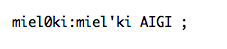
\includegraphics{presentation/img/noun-sme-lex.png}}\\
% \caption{Example of entry in the main lexicon. AIGI is the continuation class.}
% \label{nounsmelex}
% \end{center}
% \end{figure}

The main lexicon is used for analysing the student's input. We also made a smaller, pedagogical lexicon with information about the lemmas, used as a base for the quiz and grammar tasks. The lexicon should be relevant for the education in North Sámi in schools and university. 

We collected the lemmas, which were used in key textbooks for North Sámi, and added Norwegian translation, information about semantic set, dialect and inflection. We also added information about source -- which textbooks the lemma is used in. %Cf. section \ref{set} for more information about our semantic sets. 
The lexicon consists of 1538 nouns, 500 verbs and 194 adjectives, in addition to a small lexicon for grammatical word classes and numbers. Figure \ref{nounlex} shows an example of an entry in the noun lexicon. \\

\begin{figure}[tbp]
\begin{center}
\scalebox{.6}[.6]{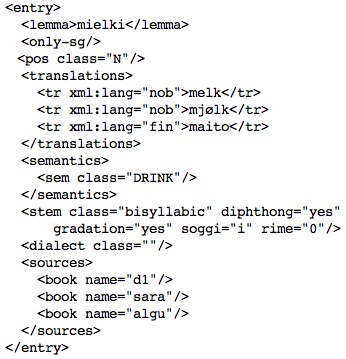
\includegraphics{presentation/img/nounlexicon3.png}}\\
\caption{An entry in the pedagogical lexicon.}
\label{nounlex}
\end{center}
\end{figure}

Some lemmas have homonymous base forms. Since they have different meanings, they belong to different semantic sets. When the student wants the translation of the lemma, it should be the translation which belongs to the particular semantic set, e.g. \textit{girdi} can be both "plane" (VEHICLE) and "pilot" (PROFESSION). Other homonomies have different inflection, and it is critical to choose the correct lemma when we are generating word forms from it, e.g. \textit{bassi} Sg Nom -- \textit{basit} Pl Nom (= holy day) and \textit{bassi} Sg Nom -- \textit{bassit} Pl Nom (= washer). We have solved the problem by giving different ids to the critical entries, e.g. id="girdi\_vehicle" vs. 
id="girdi\_profession" and id="bassi\_time" vs. id="bassi\_actor".

%It works well as long as working with semantic classes, but if the user chooses "all" or a book, then he will not understand why the program doesn't accept his suggestions, e.g. "pilot" for \textit{girdi}. The solution is that the system then looks for the lemma, instead of the id.

\subsection{Sentence generator}\label{set}
In order to be able to create a large number of potential tasks, we implemented a sentence generator. With the generator we can easily offer variation to the user, instead of tailoring every task with ready-made questions. The sentence generator is used both for generating questions and answer templates for our contextual morphology program, Morfa-C, and for generating questions to our question-answer (QA) program, Vasta. There is an example from the generator on sentence matrices in Figure \ref{questionv}.

\begin{figure}[htbp]
\begin{center}
\scalebox{.5}[.5]{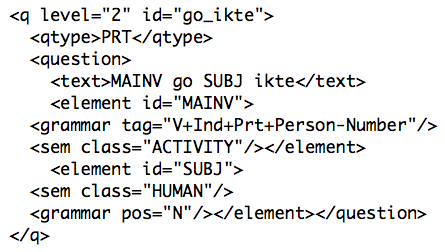
\includegraphics{presentation/img/question_vasta2.png}}\\
\caption{Example of generating if questions (MAINV question-particle SUBJ yesterday).}
\label{questionv}
\end{center}
\end{figure}

%\begin{figure}[htbp]
%\begin{center}
%\scalebox{.5}[.5]{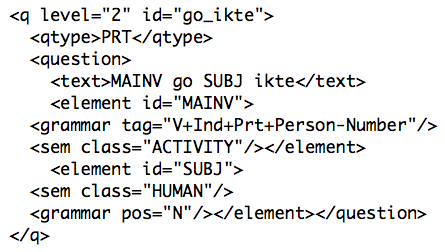
\includegraphics{presentation/img/question_vasta2.pdf}}\\
%\caption{Example of generating if questions (MAINV question-particle SUBJ yesterday).}
%\label{questionv}
%\end{center}
%\end{figure}
%
%\begin{figure}[htbp]
%\begin{center}
%\scalebox{.5}[.5]{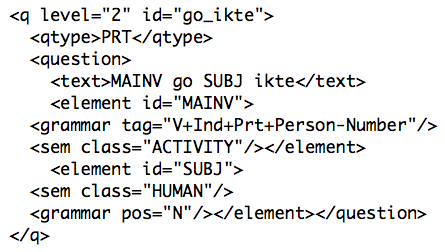
\includegraphics{presentation/img/question_vasta2.jpg}}\\
%\caption{Example of generating if questions (MAINV question-particle SUBJ yesterday).}
%\label{questionv}
%\end{center}
%\end{figure}

The question matrix contains two types of elements: constants and grammatical units. The constants such as \textit{go} and \textit{ikte} in the Figure \ref{questionv} are present in each generated sentence as such, whereas grammatical units allow more variation. Both the inflection and the content of the grammatical units may vary from question to question, and from program to program. For example, in the question in Figure \ref{questionv} the MAINV is fixed to past tense, but the person and number inflection may vary freely. In addition, certain elements such as the sentence subject (SUBJ) have default inflection in nominative, but the default inflection may be overridden. The selection of words for the sentence is constrained by semantic sets. Semantic sets are also used as an option in the word quiz. 
%There are ordinary sets and supersets, and we choose which one suits best for the particular question/task, e.g. the big superset HUMAN with all lemmas for human beings, or a smaller subset, like PROFESSION. In Figure \ref{semset} is a definition of a superset. 
%
%%sh: this figure seems to have a lot of space on the top..
%\begin{figure}[htbp]
%\begin{center}
%\scalebox{.6}[.6]{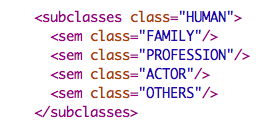
\includegraphics{presentation/img/semantic_set.png}}\\
%\caption{Some of the semantic sets are supersets, consisting of subsets. From \texttt{semantic\_sets.xml}.}
%\label{semset}
%\end{center}
%\end{figure}

The sentence generator handles agreement e.g. between subject and the main verb. The agreement may be explicitly marked between any two elements, which indicates that the two elements share the same number and person inflection.

In addition to generating questions, the sentence generator is used for generating answer templates. In this case, the sentence generator takes into account the agreement inside a sentence, but also the content and agreement between the question and the answer. For example, the person and number inflection in the answer is restricted by the question. We chose not to accept an inclusive interpretation of the pronouns in Pl1 and Du1, because we wanted the student to exercise also 2. person verb inflection. Using an inclusive interpretation, she could answer with the same verb form as in the question. Table \ref{QA} shows how the question Person-Number (QPN) Sg1 requires answer Person-Number (APN) Sg2, and so on. Pl1 as an answer to Pl1 is thus not accepted by the system.\\


\begin{table}[htdp]
\caption{Provided question-answer agreement.}
\begin{center}
\begin{tabular}[t]{ll|ll|ll}
QPN &APN &QPN &APN &QPN &APN \\
\hline
Sg1 &Sg2 &Du1 &Du2 &Pl1 &Pl2 \\
Sg2 &Sg1 &Du2 &Du1 &Pl2 &Pl1 \\
Sg3 &Sg3 &Du3 &Du3 &Pl3 &Pl3 \\
\hline
\end{tabular}
\end{center}
\label{QA}
\end{table}

\subsection{System for dialectical variation}\label{dialect}
For sentence generation the morphological generator has to be strict. This means that the generator will generate one and only one word form for every grammatical word. The analyser, on the other hand, should be tolerant (accept correct variants of the same grammatical word). Therefore we compiled two different analysers/generators, one normative but variation-tolerant transducer for analysing the input, and for sentence generation a strict one, which generates only one word form for every grammatical word.

Because of dialectical variation, we made two versions of the strict fst. We marked relevant lines in our source code in one of the following ways:

\begin{example}\label{ped}
\begin{itemize}
\item[(a)] NOT-KJ (not generate for KJ-dialect) 
\item[(b)] NOT-GG (not generate for GG-dialect)  
%\item[(c)] NG (not generate for any dialect)
\end{itemize}
\end{example}

We show an example in Figure \ref{smelex}. We also marked entries in the pedagogical lexicon-files with NOT-KJ and NOT-GG. In the makefile there are then options to generate the required dialectical variant forms of each grammatical word. This system can easily be expanded with more dialects.


\begin{figure}[htbp]
\begin{center}
\scalebox{.49}[.49]{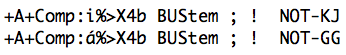
\includegraphics{presentation/img/smelex3.png}}\\
\caption{Handling of dialect variation.}
\label{smelex}
\end{center}
\end{figure}

\subsection{System for feedback on morphology}\label{mfeedback}

The information in the pedagogical lexicon about inflection is there only to give a good feedback to the student. If she doesn't inflect the lemma correctly, she can ask for hints about the inflection, and try once more, instead of getting the correct answer straight away. 

We constructed the feedback system in two steps. The first step is to define what kind of message the system should provide, based upon the combination of morphological features in the lexicon and the inflection itself. In Figure \ref{feedbacknouns} vowel change in illative Sg is defined for bisyllabic nouns which ends in the vowel \textit{i}. The message tag is used to generate the feedback to the user. 

\begin{figure}[htbp]
\begin{center}
\scalebox{.5}[.5]{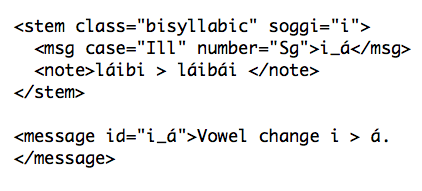
\includegraphics{presentation/img/morphfeedbackEng.png}}\\
\caption{The features in the lexicon are used to give message tags. Here the message tag is "i\_á".}
\label{feedbacknouns}
\end{center}
\end{figure}

%\begin{figure}[htbp]
%\begin{center}
%\scalebox{.55}[.55]{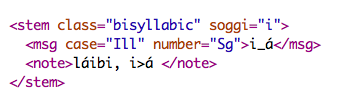
\includegraphics{presentation/img/feedback_nouns.png}}\\
%\caption{The features in the lexicon are used to give message tags. Here the message tag is "i\_á". From \texttt{feedback\_nouns.xml}.}
%\label{feedbacknouns}
%\end{center}
%\end{figure}
%
%\begin{figure}[htbp]
%\begin{center}
%\scalebox{.53}[.53]{
\includegraphics{presentation/img/messages.png}}\\
%\caption{Feedback to the user is generated from the message tags. Here for the message tag "i\_á". From \texttt{messages.xml}.}
%\label{mess}
%\end{center}
%\end{figure}
%In the example in Figures \ref{feedbacknouns}, the correct illative Sg word form of \textit{mielki} is \textit{mielkái}. %As we see in Figure \ref{nounlex}, this lemma has the feature \texttt{only-sg}, which means that we generate the lemma only in singular, even if it according to the main lexicon, also may be used in plural. This information is for pedagogical purposes; it is not that natural to use the plural form of a mass noun for a student on a lower level.

\subsection{Syntactic analyses of the student's answer} \label{sentencefeedback}
We have chosen not to use multiple-choice, but rather let the student formulate her own answer. To a certain question one may give many kinds of acceptable answers. In Sámi one may change word order, and also add many kinds of particles. 

%\textit{Maid don lohket ikte?} (What did you read yesterday?)
%\begin{itemize}
%\item \textit{Mun han lohken ollu áviissaid.} (I PART read many newspapers.)
%\item \textit{Ikte mun gal lohken buori girjji.} (Yesterday I PART read a good book.)
%\item \textit{In lohkan maidege.} (I did not read anything.)
%\item \textit{Ikte in lohkan.} (Yesterday I did not read.)
%\end{itemize}
%But the answer may contain grammar errors:
%\begin{itemize}
%\item \textit{Mun lohket ollu áviissaid.} \\ $\rightarrow$ Remember agreement between subject and verbal.  
%\item \textit{Mun lohken ollu áviissat.} \\ $\rightarrow$ There should be an accusative in your answer. 
%\item \textit{Don lohket ollu áviissaid.} \\ $\rightarrow$ Are you sure that you answer with the correct person?  
%\end{itemize}

We use vislcg3 for analysing the student's answer. The reason for choosing CG as parser platform was that only CG is robust enough for handling unconstrained input, and at the same time accurate enough to identify errors. The program contains manually written, context dependent rules, mainly used for selecting the correct analysis in case of homonymy. Each rule adds, removes, selects or replaces a tag or a set of grammatical tags in a given sentential context. Context conditions may be linked to any tag or tag set of any word anywhere in the sentence, either locally (in a fixed subdomain of the context) or globally (in the whole context). Context conditions in the same rule may be linked, i.e. conditioned upon each other, negated or blocked by interfering words or tags. Vislcg3 is documented at \cite{Visl:08}. Grammars for Danish and Norwegian based on CG achieve very good F-scores \cite{Bick:04}.

The question and the answer are merged, and given to the analyser as one text string. We use a ruleset file which disambiguates the student's input only to a certain extent, because there will probably be grammatical and orthographic errors. The last part of the file consists of rules for giving feedback to the student's grammatical errors, and rules for navigating to the correct next question of in the dialogue, due to the student's answer. How to generate feedback or navigation instructions is explained in section \ref{tutorial} and \ref{navigation}.


\begin{figure}[tbp]
\begin{center}
\scalebox{.48}[.43]{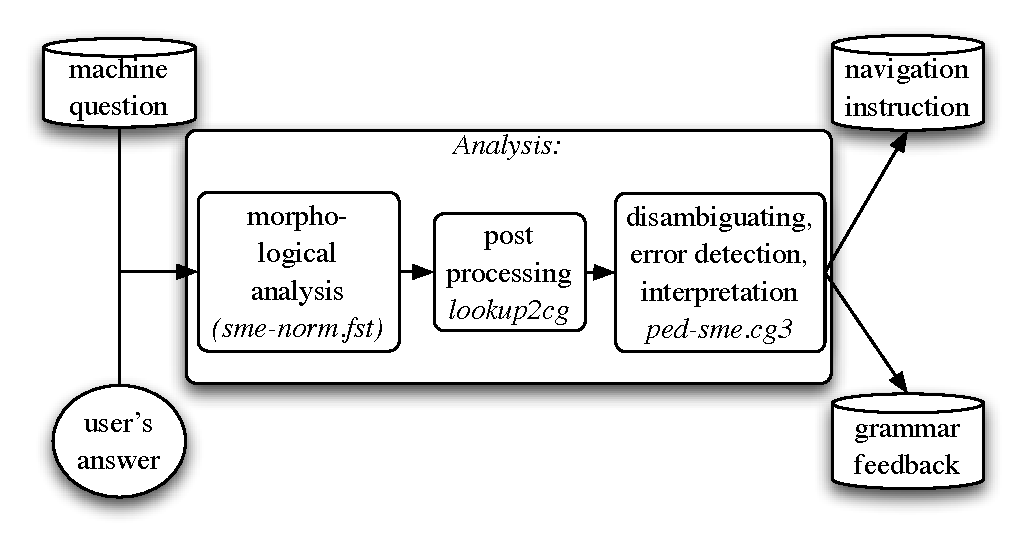
\includegraphics{presentation/img/qa2.pdf}}
\caption{An overview of the analysis process.}
\label{qasystem}
\end{center}
\end{figure}

The question mark is exchanged for a special symbol ("qst" QDL), cf. figure \ref{iktelohken}. Instead of a sentence delimiter, we want to be able to refer to the question and the answer separately in the rules.

\begin{figure}[htb]
\begin{center}
\scalebox{.53}[.45]{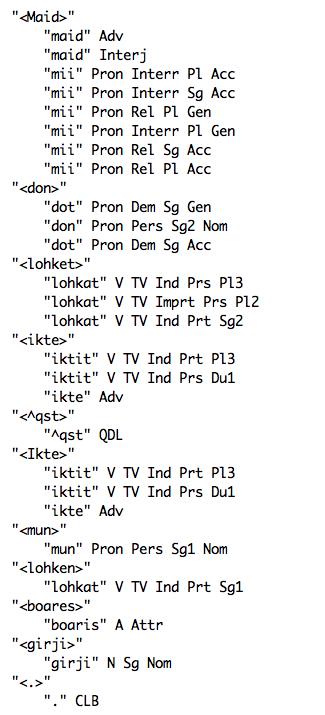
\includegraphics{presentation/img/iktelohken3.png}}
\caption{Between analysis and disambiguation.}
\label{iktelohken}
\end{center}
\end{figure}

\subsubsection{Tutorial feedback} \label{tutorial}
Tutorial feedback is feedback about grammar errors (CG prefix \textit{\&grm}), and in Figure \ref{cg3} we see a rule for assigning a tag if the student has not used accusative, when the question requires it. If the interrogative pronoun is in accusative, we expect an accusative in the answer.
%, if the question is not asking for a verb, e.g. "What do you do?" (WORK-V)
The rule assigns a \textit{\&grm-missing-Acc} tag to the interrogative pronoun if there is no accusative or negation verb in the answer.

\begin{figure}[tbp]
\begin{center}
\scalebox{.41}[.41]{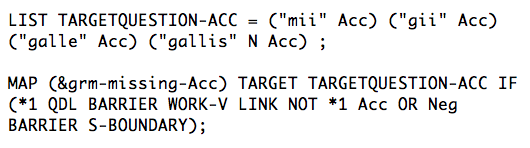
\includegraphics{presentation/img/pedcg3ny.png}}
\caption{Rule assigning missing Acc -tag.}
\label{cg3}
\end{center}
\end{figure}

Figure \ref{maidlohket} shows how the vislcg3 file has disambiguated and added the tag to the input which is the analysis from Figure \ref{iktelohken}. The tag generates feedback to the student. The object is in Nom instead of Acc, and the grammar adds the error tag.

\begin{figure}[tbp]
\begin{center}
\scalebox{.47}[.47]{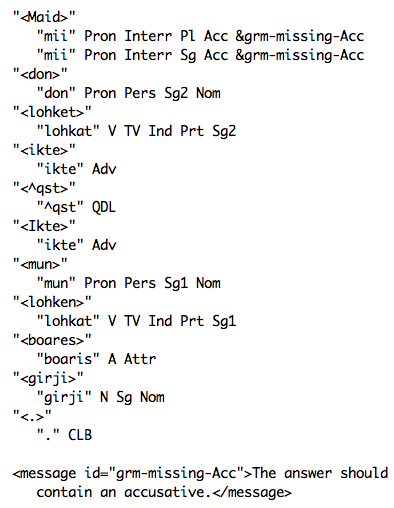
\includegraphics{presentation/img/vasta_feedback2.png}}
\caption{QA with missing Acc -tag added because the object \textit{girji} is in Nom (What did you read yesterday? Yesterday I read an old book-SgNom).}
\label{maidlohket}
\end{center}
\end{figure}

%\begin{figure}[htbp]
%\begin{center}
%\scalebox{.45}[.45]{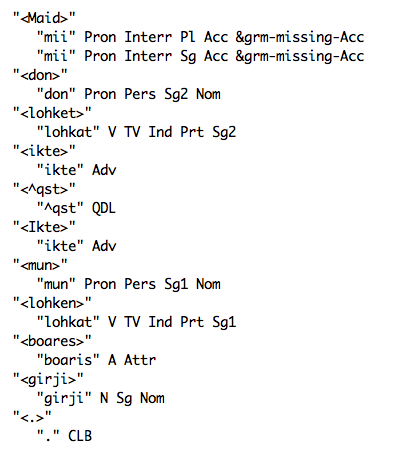
\includegraphics{presentation/img/maid_lohket_ikte3.png}}
%\caption{The grammarerrortag is added to the interrogative pronoun. (What did you read yesterday qst Yesterday I read an old book (Nom instead of Acc)). Output of vislcg3 grammar file \texttt{sme-ped.cg3}.}
%\label{maidlohket}
%\end{center}
%\end{figure}
%
%\begin{figure}[htbp]
%\begin{center}
%\scalebox{.48}[.48]{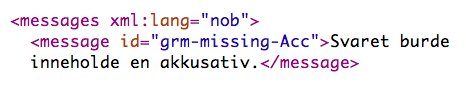
\includegraphics{presentation/img/messages_vasta2.png}}
%\caption{The grammarerrortag generates tutorial feedback. The feedback may be generated in different languages, here in Norwegian.}
%\label{messv}
%\end{center}
%\end{figure}

The biggest problem is the student's misspellings. If the spelling error gives rise to a non-existing word form, then the message to the student is \textit{The word form is not in our lexicon, can it be a spelling error?} In order to give a better feedback to certain misspellings, we have added e.g. place names with small initial letter to the fst, but with an error tag so the student gets a precise feedback. We will implement more of that kind.

The misspelling can make another word form of the same lemma. For that we make rules based on context. The real problem emerges when the spelling error gives rise to an unintended lemma. Then the challenge is to give a feedback according to what the student think s/he has written. Feedback has to be tailored from what we know about the student’s interlanguage – and we make rules for sets of typical unintended lemmas.

%\begin{itemize}
%
%\item \textbf{Locative singular without consonant gradation} \\
%The locative singular form has the suffix -s and usually consonant gradation, compared to the base form. In our pedagogical lexicon there are 1512 nouns. By adding the suffix \textit{-s} directly to the stem without consonant gradation, the result is in 57 \% of the cases a correct but unintended word form (possessive suffix in Sg3 -- e.g. \textit{viessus} instead of \textit{viesus}). Only 0,5 \% of the resulting word forms are unintended new lemmas, e.g. adverbs \textit{eanas  (eatnamis)} or verbs, e.g \textit{čogus (čohkumis)}.
%
%The possessive suffices are quite seldom used by students at lower levels, so if it does not fit to the context, one can safely assume that she has meant locative, and give feedback according to that. 
%
%\item \textbf{Illative singular without diphthong simplification and vocal change}\\
%The illative singular form has the suffix \textit{-i} or \textit{-ii} and often  diphthong simplification and vocal change. Some words have consonant gradation. By adding the suffix directly to the stem, we get 2,3 \% unintended lemmas, mostly verbs in past tense Sg3, e.g. \textit{báddii}  (pro \textit{báddái}). Generally, one man consider identifying problematic word pairs and make feedback for each of them, asking the student if she meant the other member of the pair, especially when we are not expecting one more finite verb.
%\newpage
%\item \textbf{Incorrect negative verb form}\\
%When the verb in the question is in Sg2, a common error is that the student use the Sg2 form of the verb after the negative verb, instead of the correct ConNeg form, e.g. \textit{Logat go áviissa? In logat (loga) áviissa.} The correct form is in the parentheses. The problem is that the errouneous form is a ConNeg form of another verb, \textit{logadit}, and the normal feedback will be: "You should answer with the same verb as in the question." The student will not understand this, because she thinks that the word form in the answer is an instance of the same verb. The solution was to generate all these forms of the verbs in the questions, make a set of them, and make a rule for in the right context, give the feedback: "The negative form is not correct." 
%\end{itemize}

\subsubsection{Navigating in the dialogue}\label{navigation}
We use the same system to navigate inside the dialogue. The input is tagged during analysis with information on whether it is interpreted as affirmative or negative, or with a target-tag, so that we can pick up e.g. a name or the essence of the answer, and use it in the next question or utterance. 

Some dialogues are branched according to how the student answers, e.g. if the question is about having a car, a positive answer will navigate to a branch with follow-up questions. In the same way an answer from the student about her age will induce a tag (Figure \ref{age}), which is used to navigate to different branches of the dialogue based on the age of the student, see Figure \ref{branch}.


\begin{figure}[htbp]
\begin{center}
\scalebox{.4}[.4]{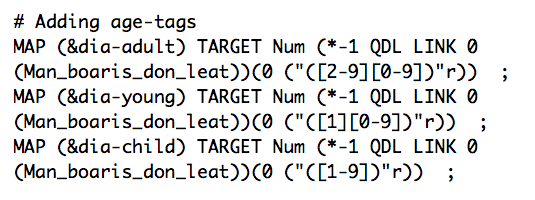
\includegraphics{presentation/img/picking_age2.png}}\\
\caption{Rules for giving age-tag to the input. Special rules for the question named Man\_boaris\_don\_leat (How\_old\_are\_you).}
\label{age}
\end{center}
\end{figure}


\begin{figure}[htbp]
\begin{center}
\scalebox{.42}[.42]{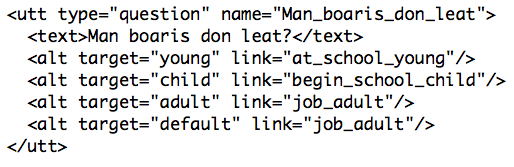
\includegraphics{presentation/img/Man_boarisEng.png}}\\
\caption{Example of how to navigate to the next question or branch, with help of the tag. The question is "How old are you?".}
% and the branches are adapted to the age of the student.}
\label{branch}
\end{center}
\end{figure}

As we see in the Figures \ref{maidlohket} and \ref{branch}, the questions in the dialogues are not generated, but written. Every question has its own unique name, so we can link to it, and it is also possible to make a rule for a special question, like in Figure \ref{age}.  

\section{The design of the programs}
The pedagogical program suite consists of six programs, cf. section 5. We will here discuss Vasta and Sahka, which utilize the syntactic analyser. 

%There are alltogehter five programs. We will here describe three of them. The other two are 
% Numra, 
%a numeral exercise based on the number word generator, and 
% Leksa, 
%a word quiz based on the pedagogical lexicon. 

%\subsection{Morfa -- word inflection}
%This is a drill made to train morphological patterns. It draws lemmas from the pedagogical lexicon at random, and the student has to answer with the word form. 

%The student can restrict the sets to certain morphosyntactic features, like Part of Speech (verbs, nouns, adjectives and numerals), and for the three first of them, it can be restricted to bisyllabic, trisyllabic and contracted stems. She can also restrict the vocabulary to certain textbooks.

%We have made two versions of the drill: Morfa-S is a bare morph-drill with singleton words. Morfa-C is a contextual morph drill, which gives matrix questions, in order to strengthen the linguistic context. After submitting the final version of the answers, the student gets a score, and a comment connected to the score.


%\subsection{Vasta -- open questions}	
\subsection{The open QA program -- Vasta}	

In between the "natural" dialogues, mimicking real life dialogues, and the pure grammar training session, inquiring paradigm forms, we have made 
%Vasta -- 
a question-answer drill. The drill has two question types: Yes/no questions and wh-questions. 

There are two motives for making this program type. First, our tailored dialogues 
%in Sahka 
run the risk of getting quickly consumed. With a QA drill we may generate an indefinite number of questions. Second, the students need to automate the question-answer routine -- inflecting the finite verb correctly and choose the correct case form.

The questions are generated, the question and answer are analysed together, and the student gets feedback, as described in \ref{sentencefeedback}. The question matrices are marked with level, so there is a level option. Only one question is presented at a time. The student can answer what she wants, but she has to use a full sentence (containing a finite verb), and use the same verb as in the question. There are 111 matrix questions divided into levels.
%\begin{itemize}
%\item Level 1: verb only in present tense, logical cases
%\item  Level 2: verb in past tense, and some verbs with oblique cases, use of postpositions, questions in which the student has to answer with case in plural,  numerals and collective numerals in nominative
%\item  Level 3: grade: numerals inflected in cases, conditional, time expressions, collective numerals
%\end{itemize}
%\vspace{0.5cm}


%\begin{figure}[htbp]
%\begin{center}
%\scalebox{.4}[.4]{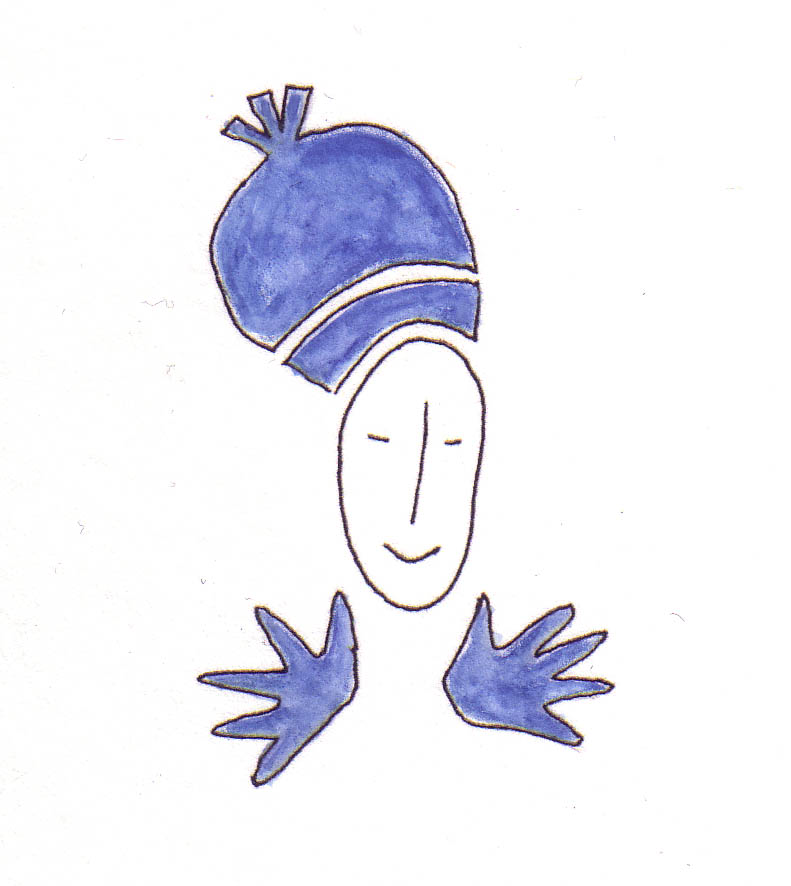
\includegraphics{presentation/img/vasta.png}}\\
%\caption{Vasta, at \textit{http://victorio.uit.no/oahpa/vasta/}}
%\label{vasta}
%\end{center}
%\end{figure}	

%\subsection{Sahka -- dialogues}
\subsection{The dialogue program -- Sahka}
The idea behind the dialogues is that the student may exercise North Sámi in a quite natural way, and at the same time get comments about errors. There will be two kinds of feedback: tags for navigation in the dialogue itself, and tags that generate tutorial feedback.

Each dialogue is made to a scenario, and each scenario has a set of underlying pedagogical goals. E.g. in the Grocery-dialogue, the scenario is a shop, and the student is telling what kind of food she wants. The underlying pedagogical goal is to exercise inflecting objects in accusative.

% \begin{figure}[htbp]
% \begin{center}
% \scalebox{.4}[.4]{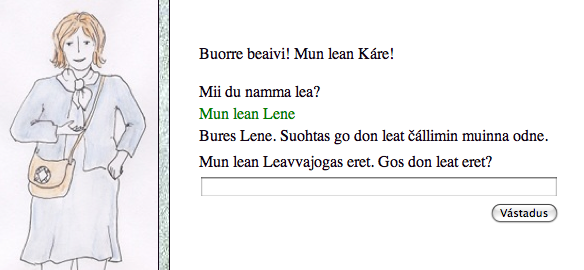
\includegraphics{presentation/img/sahka2.png}}\\
% \caption{Sahka -- the dialogue program.}
% \label{sahka}
% \end{center}
% \end{figure}

In the Get-acquainted-to-dialogues the student can choose an identity for the conversation (she chooses a picture). These identities will act as parameters for choice of comments from the computer, and for dialogue topics and dialect forms.

%\vspace{0.5cm}
%	
%Scenarios:
%\begin{itemize}
%\item Get acquainted to Hánsa -- an adult man living in Kautokeino
%\item Get acquainted to Káre -- an adult woman living in Karasjok
%\item Get acquainted to Lisa -- a girl living in Tana
%\item Get acquainted to Lemet -- a boy living in Tromsø
%\item Visit -- help to move furniture from one room to another, and have a coffee break
%\item Grocery -- buying food
%\item Comparing in the shop -- tell what is cheapest or most expensive, using adjectives in comparative or superlative
%\end{itemize}

Each dialogue consists of many branches, and different links according to the student's input. To organize them, we have made different levels:

%The first utterance is a dialogue\_opening and the last utterance is a dialogue\_closing. The student can write that she wants to quit at any point during the dialogue, and by using some form of the verb \textit{heaitit} ("quit") she will navigate directly to the dialogue\_closing.

The dialogue consists of topics, and every topic starts with an opening utterance; a comment or a question. In the end of the topic, there is always a closing.  

Every utterance has a name, and one or more links. The choice of link is dependent upon what kind of tag the question-answer pair gets, e.g. \textit{\&dia-neg} or \textit{\&dia-pos}, or \textit{\&dia-target} to a certain word, e.g. target="hivsset", like in Figure \ref{TV}.  In Figure \ref{targetIll} we see how the \textit{\&dia-target} tag is mapped to the noun in illative. There will always be a default; in case there will not be any tag. \\

\begin{figure}[htbp]
\begin{center}
\scalebox{.40}[.42]{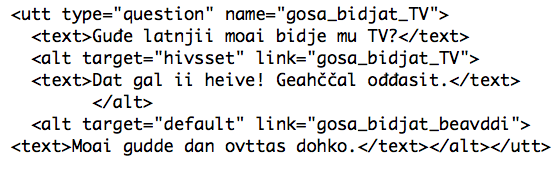
\includegraphics{presentation/img/gosabidjatTV2.png}}
\caption{The question is "In which room do we put the TV?" One of the alternatives for the navigation is due to that the target tag is put to the lemma "hivsset" ( = WC). The answer will be "That is not a good idea. Make a new try."}
\label{TV}
\end{center}
\end{figure}


\begin{figure}[htbp]
\begin{center}
\scalebox{.4}[.4]{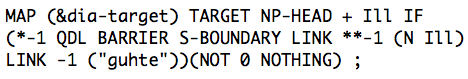
\includegraphics{presentation/img/targetIll2.png}}
\caption{A general rule, not connected to any particular question, for adding a target-tag to the NP-head in illative after a question with the interrogate \textit{guhte} + a noun in illative ( = "to which").}
%\caption{A rule for giving target-tag to an noun or pronoun in illative after a question with the interrogate \textit{guhte} + a noun in illative ( = "to which"). This a general rule, not connected to any particular question.}
\label{targetIll}
\end{center}
\end{figure}

A topic is like a module in the dialogue, and it is easy to put a new module subsequent to any topic. The linking makes it possible to make branches. Every utterance has a unique name.  

The dialogue system itself is quite simple. Only the program can make initiatives, and all the utterances from the program, are written. The program can store simple information as the student's name, place where she lives and her car type, for using in as a variable in a tailored utterance. If we were to develop the program with generating of utterances, and a more free dialogue, and also let the student take initiatives, we would have to use an analyser which maps semantic roles to the student's input, despite possible syntactic errors. In order to implement this we would need a semantically enriched lexicon.

\subsection{Web interface}

The Web framework is built on the top of a Mysql database. The information for the programs is specified in XML-documents, from where it is extracted and stored to the Mysql database. The database allows effective processing of database queries, which is crucial for real-time applications. The database also contains information outside the XML-files, such as all the inflectional forms for words in the pedagogical lexica. The basic morphological and lexicon programs exploit words from quite restricted domains. Therefore it makes sense to generate the word forms in beforehand instead of using quite heavy machinery of word form generator together with full lexica. In addition, generating the word forms and storing them to the database provides better control over the inflected word forms and e.g. different dialectal forms and thus a more stable application.

It should be noted that the dialogue and QA program use the grammatical analyser on the fly, exploiting full lexicons. This allows the user's answer to contain any North Sámi word, also words that are not restricted to the pedagogical lexicon.

\section{Evaluation}

At the time of writing, the programs have been in public use for approximately two months. % at \textit{http://oahpa.uit.no}
All user input has been logged from the very beginning, except for Vasta and Sahka, which have been logged for a couple of days only. The other programs are: Leksa -- a word quiz, Numra -- for exercising numerals, Morfa-S -- bare morphological tasks, and Morfa-C -- morphological tasks in sentential context. The log contains 32475 queries (679 queries/day for the 4 programs logged the whole period), of these, approximately 600, or under 2\%, were nonsense answers. % 4.2. - 1.4. = 8 x 7 = 42, 28507/42=679
% (of the type \textit{asdf, aaaaa}, etc.).

\begin{table}[htdp]
\caption{Answers to the programs (Vasta and Sahka were logged at the end of the period only)}
\begin{center}
\begin{tabular}{|l|r|r|r|r|}
\hline
Program     & Correct &   Wrong &    Total &  \% \\
\hline									 
Morfa-S  &  6920   & 6323    & 13243    & 52.3 \\
Leksa    &  5659   & 4248    & 9907	    & 57.1  \\
Numra    &  3086   & 2512    & 5598	    & 55.1  \\
Morfa-C  &  1349   & 1613    & 2962	    & 45.5  \\
Sahka    &   322   &   322   &  644	    & 50.0  \\
Vasta    &   19    &   102   &  121	    & 15.7 \\
\hline
Total   & 17355  &  15120  &  32475  &  53,44\\
\hline
\end{tabular}
\end{center}
\label{log1}
\end{table}

%\vspace*{-2cm}

As can be seen from table \ref{log1}, slightly more than half of the queries resulted in correct answers. When confronted with an error feedback, the user is offered grammatical help, and thereafter she has the possibility to give a new answer to the same query. An investigation of 1500 queries to Morfa-C showed that 444, or 30\%, were such repeated answers. Even though we have no log info of the use of the morphological feedback (section \ref{mfeedback}), our impression from classroom experience is that the users are actively using the feedback system. This indicates that what we are witnessing is a truly interactive process, where users err in half of the queries, and then follow up with a new try, possibly after having read the morphological advice from the program.

The error log for Sahka shows that one fourth of the errors are due to orthographical errors. Most of the "no finite verb" errors are elliptical answers, and these are not accepted, for pedagogical reasons. The remaining cases are errors where the misspelled verb is an existing word. Also for the other grammatical errors verb errors are dominating. The main goal of the program was to train verb forms in a dialogue, and the error log shows that the program is able to capture such errors.

The logs may not only be used for evaluating the programs, but also for monitoring the learning process as such. To take just one example, the Morfa logs give the error rate for each and every morphosyntactic property and stem type, thereby giving valuable information as to which parts of the verbal paradigm are the most problematic ones.

\begin{table}[htdp]
\caption{Error types for Sahka, ordered after type.}
\begin{center}
\begin{tabular}{|l|r|l|r|}
\hline
Error type & \# & Error type & \# \\
\hline												    
no finite verb    & 85 & wr. case for V-arg & 22  \\
orth. error       & 83 & wr. case after Num & 10 \\
wrong S-V agr     & 46 & wrong tense          & 9 \\
no infinite V  & 30 & no postposition      & 6 \\
wrong V choice & 24 & wrong word           & 7  \\
\hline
\end{tabular}
\end{center}
\label{log2}
\end{table}%

\section{Conclusion}

By using a sloppy version of the syntactical analyser for North Sámi, combined with a set of error-detection rules, we have been able to build a flexible CALL resource. The programs are made in a modular way, and it is easy to improve each module, and also to add more materials -- words, tasks, dialogues, levels, words from textbooks. The CG parser framework was originally chosen as parser framework for Sámi due to its extraordinary results for free-text parsing. The present project has shown that CG is well fit for making pedagogical dialogue systems as well.

The program is something quite new among pedagogical programs for Sámi, and indeed quite rare within the CALL field. %The programs are not linked to a certain chapter in a textbook, or to a certain level in the student's progression. Instead, all programs have many options, so the student can choose what to exercise, and on what level. 
The QA and the dialogue program are tolerant towards variation in student answer (not only string matching), and the random generation of tasks more or less in all of the programs, the student can use them over and over again. 



\begin{thebibliography}{}

\bibitem[\protect\citename{{Beesley and Karttunen}}2003]{BeesleyKarttunen:03}
{Kenneth R. Beesley and Lauri Karttunen}.
\newblock 2003.
\newblock {\em Finite State Morphology}.
\newblock CSLI publications in Computational Linguistics.
\newblock USA.
%Bick, Eckhard (2003-8). "A Constraint Grammar Based Question-Answering System for Portuguese". In: Fernando Moura Pires & Salvador (eds.) Progress in Artificial Intelligence (Proceedings of EPIA'2003, Beja, Dec. 2003), pp. 414-418. Springer

\bibitem[\protect\citename{Bick}2004]{Bick:04}
{Eckhard Bick}.
\newblock 2004.
\newblock {PaNoLa: Integrating Constraint Grammar and CALL}.
\newblock Henrik Holmboe (ed.): {\em Nordic Language Technology, Årbog for Nordisk Sprogteknologisk Forskningsprogram 2000-2004}.
\newblock {183--190},
\newblock Copenhagen: Museum Tusculanum.

\bibitem[\protect\citename{Bick}2005]{Bick:05}
{Eckhard Bick}.
\newblock 2005.
\newblock {Grammar for Fun: IT-based Grammar Learning with VISL}.
%\newblock {49--64},
\newblock Henriksen, Peter Juel (ed.): {\em CALL for the Nordic Languages.}
\newblock Copenhagen Studies in Language 30: 49--64.

\bibitem[\protect\citename{Gamper and Knapp}2002]{Gamper:02}
{Johann Gampfer and Judith Knapp}.
\newblock 2001.
\newblock {A review of intelligent CALL systems}.
\newblock {\em Computer Assisted Language Learning.} 
%\newblock {329--342},
\newblock {15(4): 329--342.}
%\newblock Routledge.


\bibitem[\protect\citename{Heift}2001]{Heift:01}
{Trude Heift}.
\newblock 2001.
\newblock {Intelligent Language Tutoring Systems for Grammar Practice}.
\newblock {\em Zeitschrift fur Interkulturellen Fremdsprachenunterricht [Online] }
\newblock {6(2).}



\bibitem[\protect\citename{Heift and Nicholson}2001]{Heift:02}
{Trude Heift and Devlan Nicholson}.
\newblock 2001.
\newblock {Web Delivery of Adaptive and Interactive Language Tutoring}.
%\newblock {310--325},
\newblock {\em International Journal of Artificial Intelligence in Education.}
\newblock {12(4): 310--325.}

\bibitem[\protect\citename{Heift and Schulze}2007]{Heift:07}
{Trude Heift and Mathias Schulze}.
\newblock 2007.
\newblock {\em Errors and intelligence in computer-assisted language learning: parsers and pedagogues}.
\newblock Routledge studies in computer-assisted language learning 2. 
\newblock New York : Routledge.

\bibitem[\protect\citename{Karlsson et. al}1995]{Karlsson:95}
{Fred Karlsson and Atro Voutilainen and Juha Heikkilä and Arto Anttila}.
\newblock 1995.
\newblock {\em Constraint grammar: a language-independent system for parsing unrestricted text}.
\newblock Mouton de Gruyter.


%\bibitem[\protect\citename{Samuelsson and Voutilainen}1997]{SamuelssonVoutilainen:97}
%{Christer Samuelsson and Atro Voutilainen}.
%\newblock 1997.
%\newblock Comparing a Linguistic and a Stochastic Tagger
%\newblock {\em Proceedings of the 35th Annual Meeting of the Association for Computational Linguistics}.
%\newblock {Association for Computational Linguistics},
%\newblock {246--253},
%\newblock {http://www.aclweb.org/anthology/P97-1032}


\bibitem[\protect\citename{{Trosterud}}2007]{Trosterud:07}
{Trond Trosterud}.
\newblock 2007.
\newblock {\em Language technology for endangered languages: Sámi as a case study}.
\newblock http://giellatekno.uit.no/background/rvik.pdf
\newblock University of Tromsø, Norway.

\bibitem[\protect\citename{{visl}}2008]{Visl:08}
{VISL-group}.
\newblock 2008.
\newblock {\em Constraint Grammar}.
\newblock http://beta.visl.sdu.dk/constraint\_grammar.html
%\newblock Institute of Language and Communication (ISK), 
\newblock University of Southern Denmark.


\end{thebibliography}


%\begin{spacing}{1}
%\par
%\bibliographystyle{jmr} %jmr gives the second author with first name first
%\bibliographystyle{jmr}
%\thebibliography{refacl}
%\bibliographystyle{acl}


%\bibdata{refacl}
%\addcontentsline{toc}{section}{References}
%\end{spacing}

	
\end{document}

	
